\PassOptionsToPackage{unicode=true}{hyperref} % options for packages loaded elsewhere
\PassOptionsToPackage{hyphens}{url}
\PassOptionsToPackage{dvipsnames,svgnames*,x11names*}{xcolor}
%
\documentclass[10pt,ignorenonframetext,]{beamer}
\usepackage{pgfpages}
\setbeamertemplate{caption}[numbered]
\setbeamertemplate{caption label separator}{: }
\setbeamercolor{caption name}{fg=normal text.fg}
\beamertemplatenavigationsymbolsempty
% Prevent slide breaks in the middle of a paragraph:
\widowpenalties 1 10000
\raggedbottom
\setbeamertemplate{part page}{
\centering
\begin{beamercolorbox}[sep=16pt,center]{part title}
  \usebeamerfont{part title}\insertpart\par
\end{beamercolorbox}
}
\setbeamertemplate{section page}{
\centering
\begin{beamercolorbox}[sep=12pt,center]{part title}
  \usebeamerfont{section title}\insertsection\par
\end{beamercolorbox}
}
\setbeamertemplate{subsection page}{
\centering
\begin{beamercolorbox}[sep=8pt,center]{part title}
  \usebeamerfont{subsection title}\insertsubsection\par
\end{beamercolorbox}
}
\AtBeginPart{
  \frame{\partpage}
}
\AtBeginSection{
  \ifbibliography
  \else
    \frame{\sectionpage}
  \fi
}
\AtBeginSubsection{
  \frame{\subsectionpage}
}
\usepackage{lmodern}
\usepackage{amssymb,amsmath}
\usepackage{ifxetex,ifluatex}
\usepackage{fixltx2e} % provides \textsubscript
\ifnum 0\ifxetex 1\fi\ifluatex 1\fi=0 % if pdftex
  \usepackage[T1]{fontenc}
  \usepackage[utf8]{inputenc}
  \usepackage{textcomp} % provides euro and other symbols
\else % if luatex or xelatex
  \usepackage{unicode-math}
  \defaultfontfeatures{Ligatures=TeX,Scale=MatchLowercase}
\fi
\usetheme[]{Singapore}
\usefonttheme{serif}
% use upquote if available, for straight quotes in verbatim environments
\IfFileExists{upquote.sty}{\usepackage{upquote}}{}
% use microtype if available
\IfFileExists{microtype.sty}{%
\usepackage[]{microtype}
\UseMicrotypeSet[protrusion]{basicmath} % disable protrusion for tt fonts
}{}
\IfFileExists{parskip.sty}{%
\usepackage{parskip}
}{% else
\setlength{\parindent}{0pt}
\setlength{\parskip}{6pt plus 2pt minus 1pt}
}
\usepackage{xcolor}
\usepackage{hyperref}
\hypersetup{
            pdftitle={Klyngeanalyse},
            pdfauthor={Stefanie Muff, Institutt for matematiske fag},
            colorlinks=true,
            linkcolor=Maroon,
            filecolor=Maroon,
            citecolor=Blue,
            urlcolor=blue,
            breaklinks=true}
\urlstyle{same}  % don't use monospace font for urls
\newif\ifbibliography
\usepackage{graphicx,grffile}
\makeatletter
\def\maxwidth{\ifdim\Gin@nat@width>\linewidth\linewidth\else\Gin@nat@width\fi}
\def\maxheight{\ifdim\Gin@nat@height>\textheight\textheight\else\Gin@nat@height\fi}
\makeatother
% Scale images if necessary, so that they will not overflow the page
% margins by default, and it is still possible to overwrite the defaults
% using explicit options in \includegraphics[width, height, ...]{}
\setkeys{Gin}{width=\maxwidth,height=\maxheight,keepaspectratio}
\setlength{\emergencystretch}{3em}  % prevent overfull lines
\providecommand{\tightlist}{%
  \setlength{\itemsep}{0pt}\setlength{\parskip}{0pt}}
\setcounter{secnumdepth}{0}

% set default figure placement to htbp
\makeatletter
\def\fps@figure{htbp}
\makeatother

\usepackage{multicol}

\title{Klyngeanalyse}
\providecommand{\subtitle}[1]{}
\subtitle{ISTx1003 Statistisk læring og Data Science}
\author{Stefanie Muff, Institutt for matematiske fag}
\date{November 12, 2021}

\begin{document}
\frame{\titlepage}

\begin{frame}{Plan for i dag}
\protect\hypertarget{plan-for-i-dag}{}

\(~\)

\begin{itemize}
\item
  Hva er klyngeanalyse
\item
  Læringsmål, pensum og læringsressurser
\item
  Avstandsmål
\item
  K-gjennomsnitt (``K-means'') klyngeanalyse
\item
  Bruk av klyngeanalyse på et bilde (prosjektet fra i fjor)
\item
  Hierarkisk klyngeanalyse
\item
  Informasjon om prosjektet
\end{itemize}

\end{frame}

\begin{frame}{Eksempel 1: Genaktivitet}
\protect\hypertarget{eksempel-1-genaktivitet}{}

\begin{itemize}
\item
  \(n=81\) celleprøver fra kreftsvulster til ulike pasienter
\item
  genaktivitet for \(p =12957\) gener
\end{itemize}

\vspace{2mm}

\textbf{Spørsmål:}

Hvilke celleprøver fra brystkreftpasienter ligner hverandre mest?

Kan vi finne ukjente klynger (av celleprøver) i dataene?

Dette kan hjelpe for å forutsi sannsynlighet for en tilbakefall.

\end{frame}

\begin{frame}

\centering

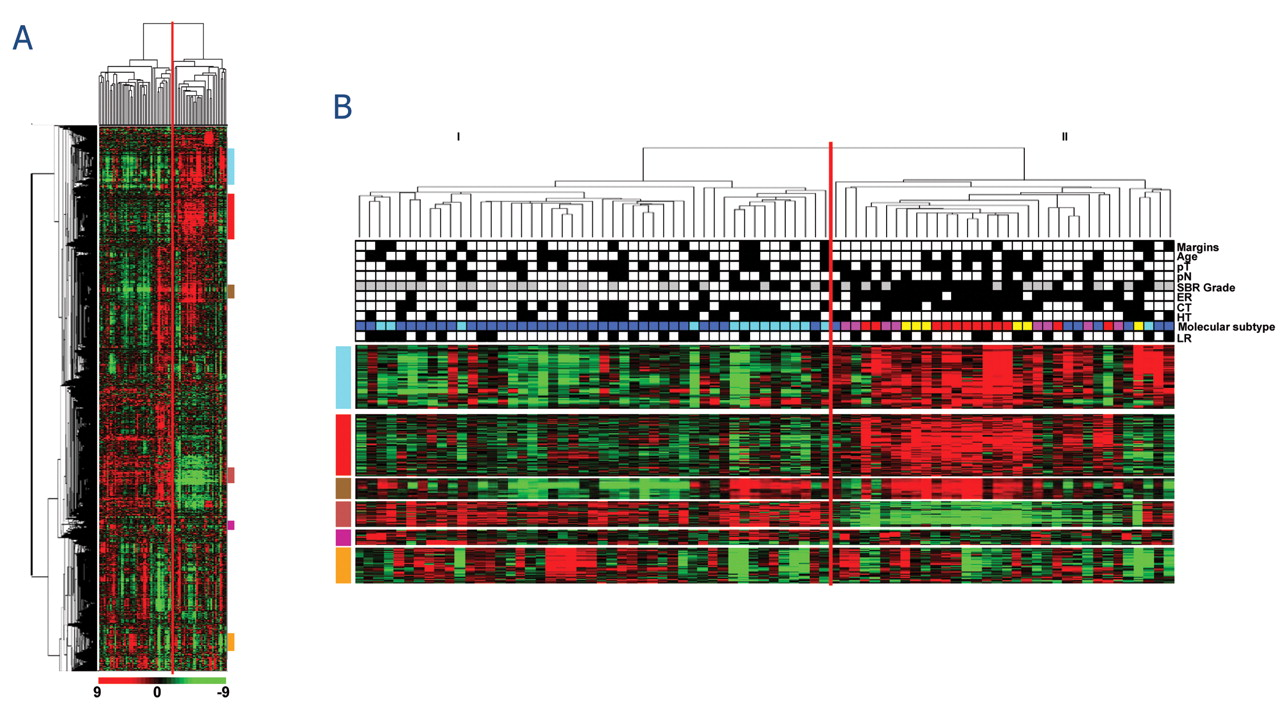
\includegraphics[width=0.9\textwidth,height=\textheight]{gene_expression.jpg}
\[ X = p\times n  =  \text{gener} \times \text{prøver}  \ .\]

\tiny

Finn ut mer: \url{https://cgp.iiarjournals.org/content/8/4/199}

\end{frame}

\begin{frame}{Eksempel 2: Proteininteraksjonsnettwerk}
\protect\hypertarget{eksempel-2-proteininteraksjonsnettwerk}{}

Kan vi finne klynger med relatert funksjon?

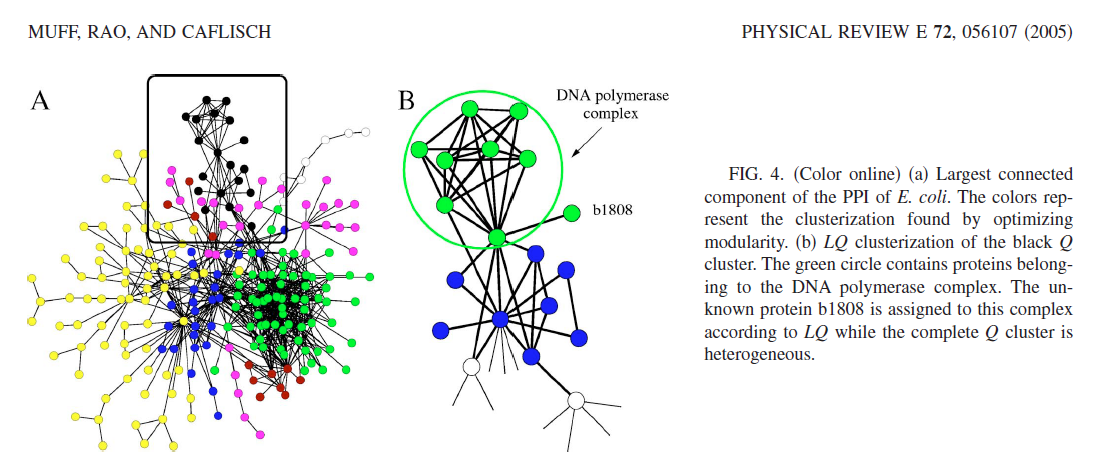
\includegraphics{muff_etal.png}

\end{frame}

\begin{frame}{Læringsmål}
\protect\hypertarget{luxe6ringsmuxe5l}{}

\begin{itemize}
\item
  forstå hvorfor det er interessant å gjøre klyngeanalyse
\item
  kjenne igjen situasjoner der klyngeanalyse vil være en aktuell metode
  å bruke
\item
  kjenne begrepene avstandsmål, koblingstype, dendrogram
\item
  forstå algoritmen for å utføre K-gjennomsnitt-klyngeanalyse og
  hierarkisk klyngeanalyse
\item
  forstå hvordan klyngeanalyse utføres i Python
\item
  kunne besvare oppgave 3 av prosjektoppgaven på en god måte!
\end{itemize}

\end{frame}

\begin{frame}{Læringsressurser}
\protect\hypertarget{luxe6ringsressurser}{}

\vspace{2mm}

\(~\)

Tema Klyngeanalyse:

\vspace{2mm}

\begin{itemize}
\item
  \textbf{Kompendium}: Klyngeanalyse (pdf og html, by Mette Langaas)
\item
  \textbf{Korte videoer}: (by Mette Langaas)

  \begin{itemize}
  \tightlist
  \item
    Klyngeanalyse (8:43 min)
  \item
    Hierarkisk klyngeanalyse (11:26 min)
  \item
    K-gjennomsnitt-klyngeanalyse (8:38 min)
  \end{itemize}
\item
  Denne forelesningen
\item
  \textbf{Disse slides} med notater
\end{itemize}

\(~\)

\url{https://wiki.math.ntnu.no/istx1003/2021h/start}

\end{frame}

\begin{frame}{Klyngeanalyse -- hva er det?}
\protect\hypertarget{klyngeanalyse-hva-er-det}{}

\begin{itemize}
\item
  Mål:

  \begin{itemize}
  \item
    tilordne en ny observasjon til en av flere \emph{kjente} klasser
  \item
    lage en klassifikasjonsregel
  \item
    estimere sannsynligheten for at en ny observasjon tilhører de ulike
    klassene
  \end{itemize}
\end{itemize}

\vspace{2mm}

For hver av de uavhengige observasjonene \(i=1,\ldots,n\) har vi

\begin{itemize}
\tightlist
\item
  Forklaringsvariabler \((x_{1i},x_{2i},\ldots,x_{pi})\)
\item
  En kategorisk responsvariablel \(y_i\).
\end{itemize}

\end{frame}

\begin{frame}

\begin{block}{Eksempler}

\end{block}

\end{frame}

\end{document}
